\begin{comment}
    Introducción
        XAI y las distintas métricas que existen
            Feature attribution, counterfactual, rule based, sufficient reason, etc
        Algoritmos de feature attribution
        Código fuente 
\end{comment}

Las capacidades de los distintos modelos de inteligencia artificial (IA) han ido creciendo exponencialmente en los últimos años. Tareas que creíamos imposibles de realizar a través de estas técnicas, como la resolución de problemas matemáticos complejos, hoy en día pueden ser resueltas por los LLMs \cite{frontierMath}. No sólo aumentó la complejidad de las tareas que pueden resolver, sino también la complejidad de sus arquitecturas y de como están compuestos. Los modelos de hace unos años tenían 1e8 parámetros, mientras que hoy en día ya llegan a 1e12. \cite{EpochLargeScaleModels2024}. El problema que esto genera es que cada vez es más difícil entender como funcionan y como obtienen las respuestas que nos dan. Esto es algo sumamente importante, ya que si uno está utilizando estas técnicas para diagnósticos médicos u otras situaciones igual de delicadas, es fundamental  entender como los modelos alcanzan sus conclusiones . Ahí es donde entra en juego el área de XAI, Explainable Artificial Intelligence.

El objetivo principal de esta área de investigación consiste en encontrar una explicación para las decisiones o predicciones de los distintos modelos de IA, para poder entender el razonamiento detrás de las mismas. Dentro de esta área hay dos ramas principales, la explicabilidad y la interpretabilidad. La primera se centra en obtener estas explicaciones, y es el área en la cual nos centramos en este trabajo. La segunda en entender a los modelos y su representación interna \cite{interpretabilityPaper}. Estas explicaciones no son útiles únicamente en tanto permiten que los usuarios entiendan el porqué de la respuesta, sino también debido a que ayudan a detectar errores o sesgos indeseados que se hayan generado durante el entrenamiento. 

Dentro del área de explicabilidad hay varios tipos de métodos \cite{interpretabilityBook}, los cuales pueden agruparse de acuerdo a distintos ejes:
\begin{itemize}
    \item \textit{Modelo}
        \begin{itemize}
            \item Agnóstico: Son los métodos que se pueden aplicar a todo tipo de modelos. Por ejemplo en SHAP, el método que describiremos más adelante, su valor no depende de la implementación interna del modelo. %\santi{A qué te referís acá?} 
            \item Específico: Son los métodos que tienen una implementación que está acoplada al modelo que buscan explicar, como en el caso de \textit{Tree-Shap}, que en su implementación se utilizan los caminos del árbol para calcular su valor, aprovechando propiedades de la estructura del modelo.
            %\santi{Acá creo que sería mejor usar como ejemplo que en el caso de árboles podés tomar el camino como justificación. Eso es claramente único al modelo, mientras que Tree-shap es un concepto agnóstico al modelo pero que se calcula de forma piola en árboles.} 
        \end{itemize}
    \item \textit{Alcance}
        \begin{itemize}
            \item Explicación global: Busca descubrir cualidades o comportamientos que el modelo tenga en todas sus predicciones. Por ejemplo, para entender por qué un modelo le otorga un préstamo a un individuo, se observa que el nivel de ingresos siempre es un feature relevante. %.\santi{Acá siento que queda medio vago lo de explicar en su totalidad. Una alternativa es "busca descubrir cualidades o comportamientos que el modelo tenga en todas sus predicciones, como por ejemplo si el modelo mira o no la cantidad de metros cuadrados de una casa, pensando en los datasets de Housing".}
            \item Explicación local: Busca descubrir cualidades o comportamiento que el modelo tenga para un conjunto reducido de instancias del dataset. Por ejemplo, para entender por qué un modelo le otorga un préstamo a un individuo, podemos encontrar que para las personas casadas, la cantidad de hijos es un feature que toma más relevancia.  %\santi{Idem anterior, ser mas precisos y ejemplificar.}
        \end{itemize}
    \item \textit{Tipo de explicación:} Hay varias categorías del tipo de explicación que puede tener un método, por ejemplo \textit{feature importance}, el cual asigna valores a cada feature. También hay \textit{interpretaciones visuales} como saliency maps o correlations plots. Incluso hay métodos que generan un modelo más simple a partir del modelo original, como \textit{Lime}. 

    Cabe destacar que no existe un consenso absoluto sobre qué constituye una "explicación" en el contexto de la inteligencia artificial. Muchas de las técnicas mencionadas —como feature attribution o interpretaciones visuales— son aproximaciones pragmáticas a un problema mucho más amplio y complejo, vinculado a cuestiones filosóficas sobre comprensión, causalidad e interpretación humana \cite{MILLER20191, lipton2017mythosmodelinterpretability}. En este sentido, lo que hoy se considera una explicación en XAI responde más a criterios de utilidad y simplicidad interpretativa que a una definición formal y universalmente aceptada.

    %\santi{Ojo que está incompleto. Btw, en esta parte podrías agregar un párrafo cuestionando qué es una explicación, y podemos buscar citas a discusiones más filosóficas. Onda, que quede claro que feature attribution y etc son una aproximación a una ambición filosófica mucho mayor.}\sergio{agreed}
\end{itemize}

En esta tesis nos centramos en \textit{SHAP} \cite{shapOriginalPaper}, el cual es un método que, en principio, provee explicaciones agnósticas al modelo, con un alcance local y que es del tipo de feature attribution. Esto significa que para una predicción individual que realiza el modelo, \textit{SHAP} va a devolver un valor asociado a cada feature de la instancia. Decimos que es agnóstico, puesto que su valor depende meramente del ouput del modelo, por lo que no esta acoplado a su representación interna. Aún así, \textit{SHAP} actualmente es un framework que engloba varios tipos de métodos, ya que hay distintas aproximaciones según cuál sea tu tipo de modelo. Por ejemplo, existen métodos como DeepExplainer, TreeExplainer y LinearExplainer dentro del  \textcolor{blue}{\href{https://shap.readthedocs.io/en/latest/index.html}{framework}}  SHAP, los cuales se utilizan para modelos específicos, pero también hay otros métodos como KernelExplainer, que son agnósticos al modelo.

%\santi{Pero no es este el motivo por el cual decimos que es agnóstico, no? Decimos que es agnóstico porque su valor depende únicamente del mappeo de entradas a salidas. O sea, es una propiedad del mappeo subyacente al modelo, ignorando la arquitectura específica. Entiendo que la idea original es esa, y estas versiones que se nombras después son aproximaciones imperfectas (pq muchas veces nisiquiera coinciden con los shapley o SHAP) para modelos particulares.}

Uno de los problemas principales de este framework es lo costoso que es calcularlo, y en particular, hay estudios que analizan esta dificultad desde el punto de vista de la complejidad computacional. Por ejemplo, se demostró que calcular SHAP para un clasificador trivial era NP-completo, o intratable, para datos con distribuciones más o igual de complejas que una Naive Bayes \cite{arenas2021tractability}.
A raíz de esto, nos resultó interesante analizar si existía alguna variación de SHAP, la cual pueda ser calculada en tiempo polinomial para una distribución de red bayesiana. Además, actualmente hay trabajos similares a este, que buscan analizar la complejidad de SHAP según la variante, el modelo y la distribución \cite{marzouk2025computationaltractabilitymanyshapley} %\santi{Hace poco salió este paper, habría que agregarlo en algún lado -> On the Computational Tractability of the (Many) Shapley Values} 

SHAP está basado en los Shapley values \cite{shapley1953value}, un valor de teoría de juegos.  Una variación de los mismos son los assymetric shapley values (ASV), los cuales pueden introducir el factor de causalidad al cálculo de los mismos. De esta manera, se define ASV \cite{frye2019asymmetric}, un framework similar a SHAP, el cual además tiene en cuenta el grafo causal de los datos. El objetivo es esta tesis es lograr calcular ASV en tiempo polinomial de forma exacta y aproximada para datos con distribuciones de redes bayesianas.

\subsection{Explicaciones basadas en causalidad: Un ejemplo comparativo entre SHAP y ASV} \label{asvCaseExample}
\echu{¿Juega el ejemplo así?}

En esta sección presentamos un ejemplo tomado de la sección 4.1 del artículo original de ASV \cite{frye2019asymmetric}, con el objetivo de ilustrar como la incorporación de información causal puede enriquecer las explicaciones de un modelo. Se utiliza como caso de estudio datos del conjunto Census Income de la UCI \cite{dua2017uci}, en el cual se entrena un modelo (en este caso una red neuronal) para predecir si el ingreso de un individuo supera los \$50\,000. Dado que algunas de las variables demográficas presentes en este conjunto (por ejemplo, la edad) son claramente causas de otras (por ejemplo, el nivel educativo), es especialmente pertinente considerar información causal al interpretar la predicción del modelo. El conjunto $A$ son las variables definidas como los ancestros causales, con $A= \set{age, sex, native \ country, race}$ y el resto de variables son descendientes de estas, dentamos a los descendientes como el conjunto $D$. 

Para este experimento se calculan dos variaciones de SHAP, una \emph{off-manifold} y otra \emph{on-manifold}, la diferencia es la función de probabilidad que ambas usan. En el enfoque \emph{on-manifold} se respetan las restricciones que hay entre las distintas variables, por ejemplo a la hora de calcular SHAP se va a descartar cualquier instancia tal que $age=3 \land occupation = teacher$, ya que eso no es posible. Pero en el enfoque \emph{off-manifold} no va a haber ninguna restricción a la hora de combinar los distintos valores de cada feature. 

\begin{figure}
    \centering
    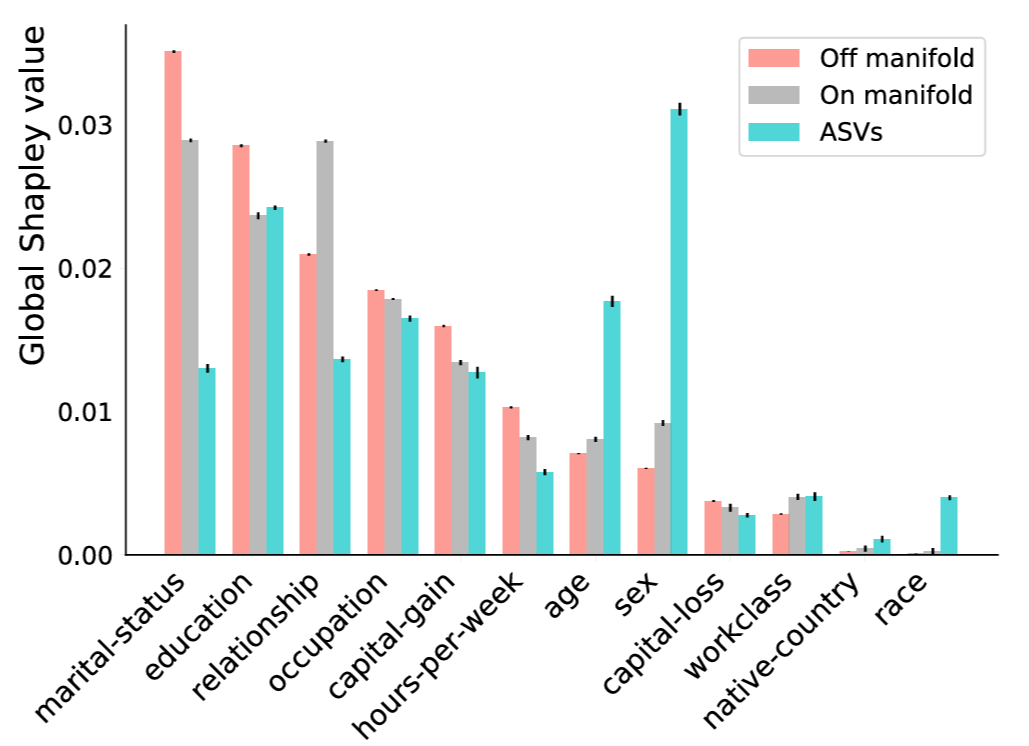
\includegraphics[width=0.5\linewidth]{img/asvPaperPlotExample.png}
    \caption{Valores globales de los Shapley Values y ASV para el modelo entrenado para el Census Income dataset.}
    \label{fig:asvPaperPlotExample}
\end{figure}

La Figura \ref{fig:asvPaperPlotExample} muestra como la variable \emph{género} presenta un Shapley value relativamente pequeño en el análisis off-manifold. En cambio, al incorporar el conocimiento causal mediante ASV, se observa que dicha variable recibe un valor significativamente mayor. Este hallazgo evidencia que, a pesar de que el género tenga una influencia moderada en el modelo cuando se considera de forma aislada, su papel en la explicación se amplifica una vez que se tiene en cuenta su relación causal con otras variables (como el estado civil o la relación actual). De esta forma, los ASVs proporcionan una medida más precisa y contrastada de la contribución de cada variable, permitiendo detectar aspectos de discriminación o sesgo que de otro modo pasarían desapercibidos.

Este ejemplo evidencia cuándo es útil incorporar información causal en la explicación de modelos: en situaciones donde se conoce una relación de causa y efecto entre las variables, el uso de ASVs no solo mejora la interpretabilidad de la explicación, sino que también aporta una perspectiva más fiel al proceso generador de los datos, contribuyendo así a la construcción de modelos más transparentes y confiables.

%\sergio{En general me parece que hay que poner más motivación y ejemplos en esta sección. Estos también pueden servir para ser referenciados y hacer más concretos los conceptos que se introducen después, como ser en la sección 2.}

%\santi{Agreed. Haría un ejemplito con una predicción, y un típico gráfico de esos que muestran los SHAP scores. Idealmente es un ejemplo donde por no tener cuenta correlaciones se asignan mal los scores. Dps cuando introducis ASV mostras que usando la red causal mejora el ranking (i.e. refleja mejor la importancia de los features)}


\subsection{Código fuente}

Todos los algoritmos presentados en este trabajo fueron implementados. El código fuente puede ser encontrado online en el siguiente repositorio: 

\begin{table}[H]
\centering
\begin{tabular}{ll}
\toprule
\textbf{Repository} & \textbf{Repository} \\
\midrule
Source code & \url{https://github.com/EchuCompa/pasantia-BICC} \\
\end{tabular}
\end{table}